Il est pertinent de chercher à comprendre quelle couche morphologique, parmi les trois introduites dans la partie précédente, est la plus efficace pour à la fois apprendre automatiquement et effectuer de manière précise une des deux opérations morphologiques fondamentales (érosion et dilatation), dans un réseau de neurones. Pour ce faire, l'étude se fait à partir de l'analyse de la convergence et de l'état final des réseaux de neurones morphologiques construits suivant l'architecture fig. \ref{fig:architecture_reseau_morpho}. La comparaison de l'efficacité des trois différents types de réseaux morphologiques ($p$ConvNet, $\mathcal{L}$MorphNet et $\mathcal{S}$MorphNet), se fait suivant les 4 groupes décrits précédemment selon le type d'opération cible (érosion, dilatation, ouverture, fermeture). \\

\vspace{-1.0mm}
\noindent En reprenant les résultats de recherche de Hermary et al. \cite{Hermary_2022}, on obtient les résultats de convergence et de métriques ainsi que les figures présentés dans cette sous-partie. \\

\vspace{0.0mm}
Dans le premier cas, i.e. pour une opération d'érosion avec un réseau à 1 couche morphologique, on obtient les résultats de convergence et de caractéristiques suivants, sur 5 runs par expérience, fig \ref{fig:art_resultats_erosion} :

% figure
\vspace{5.0mm}
\begin{figure}[ht]
  \begin{center}
    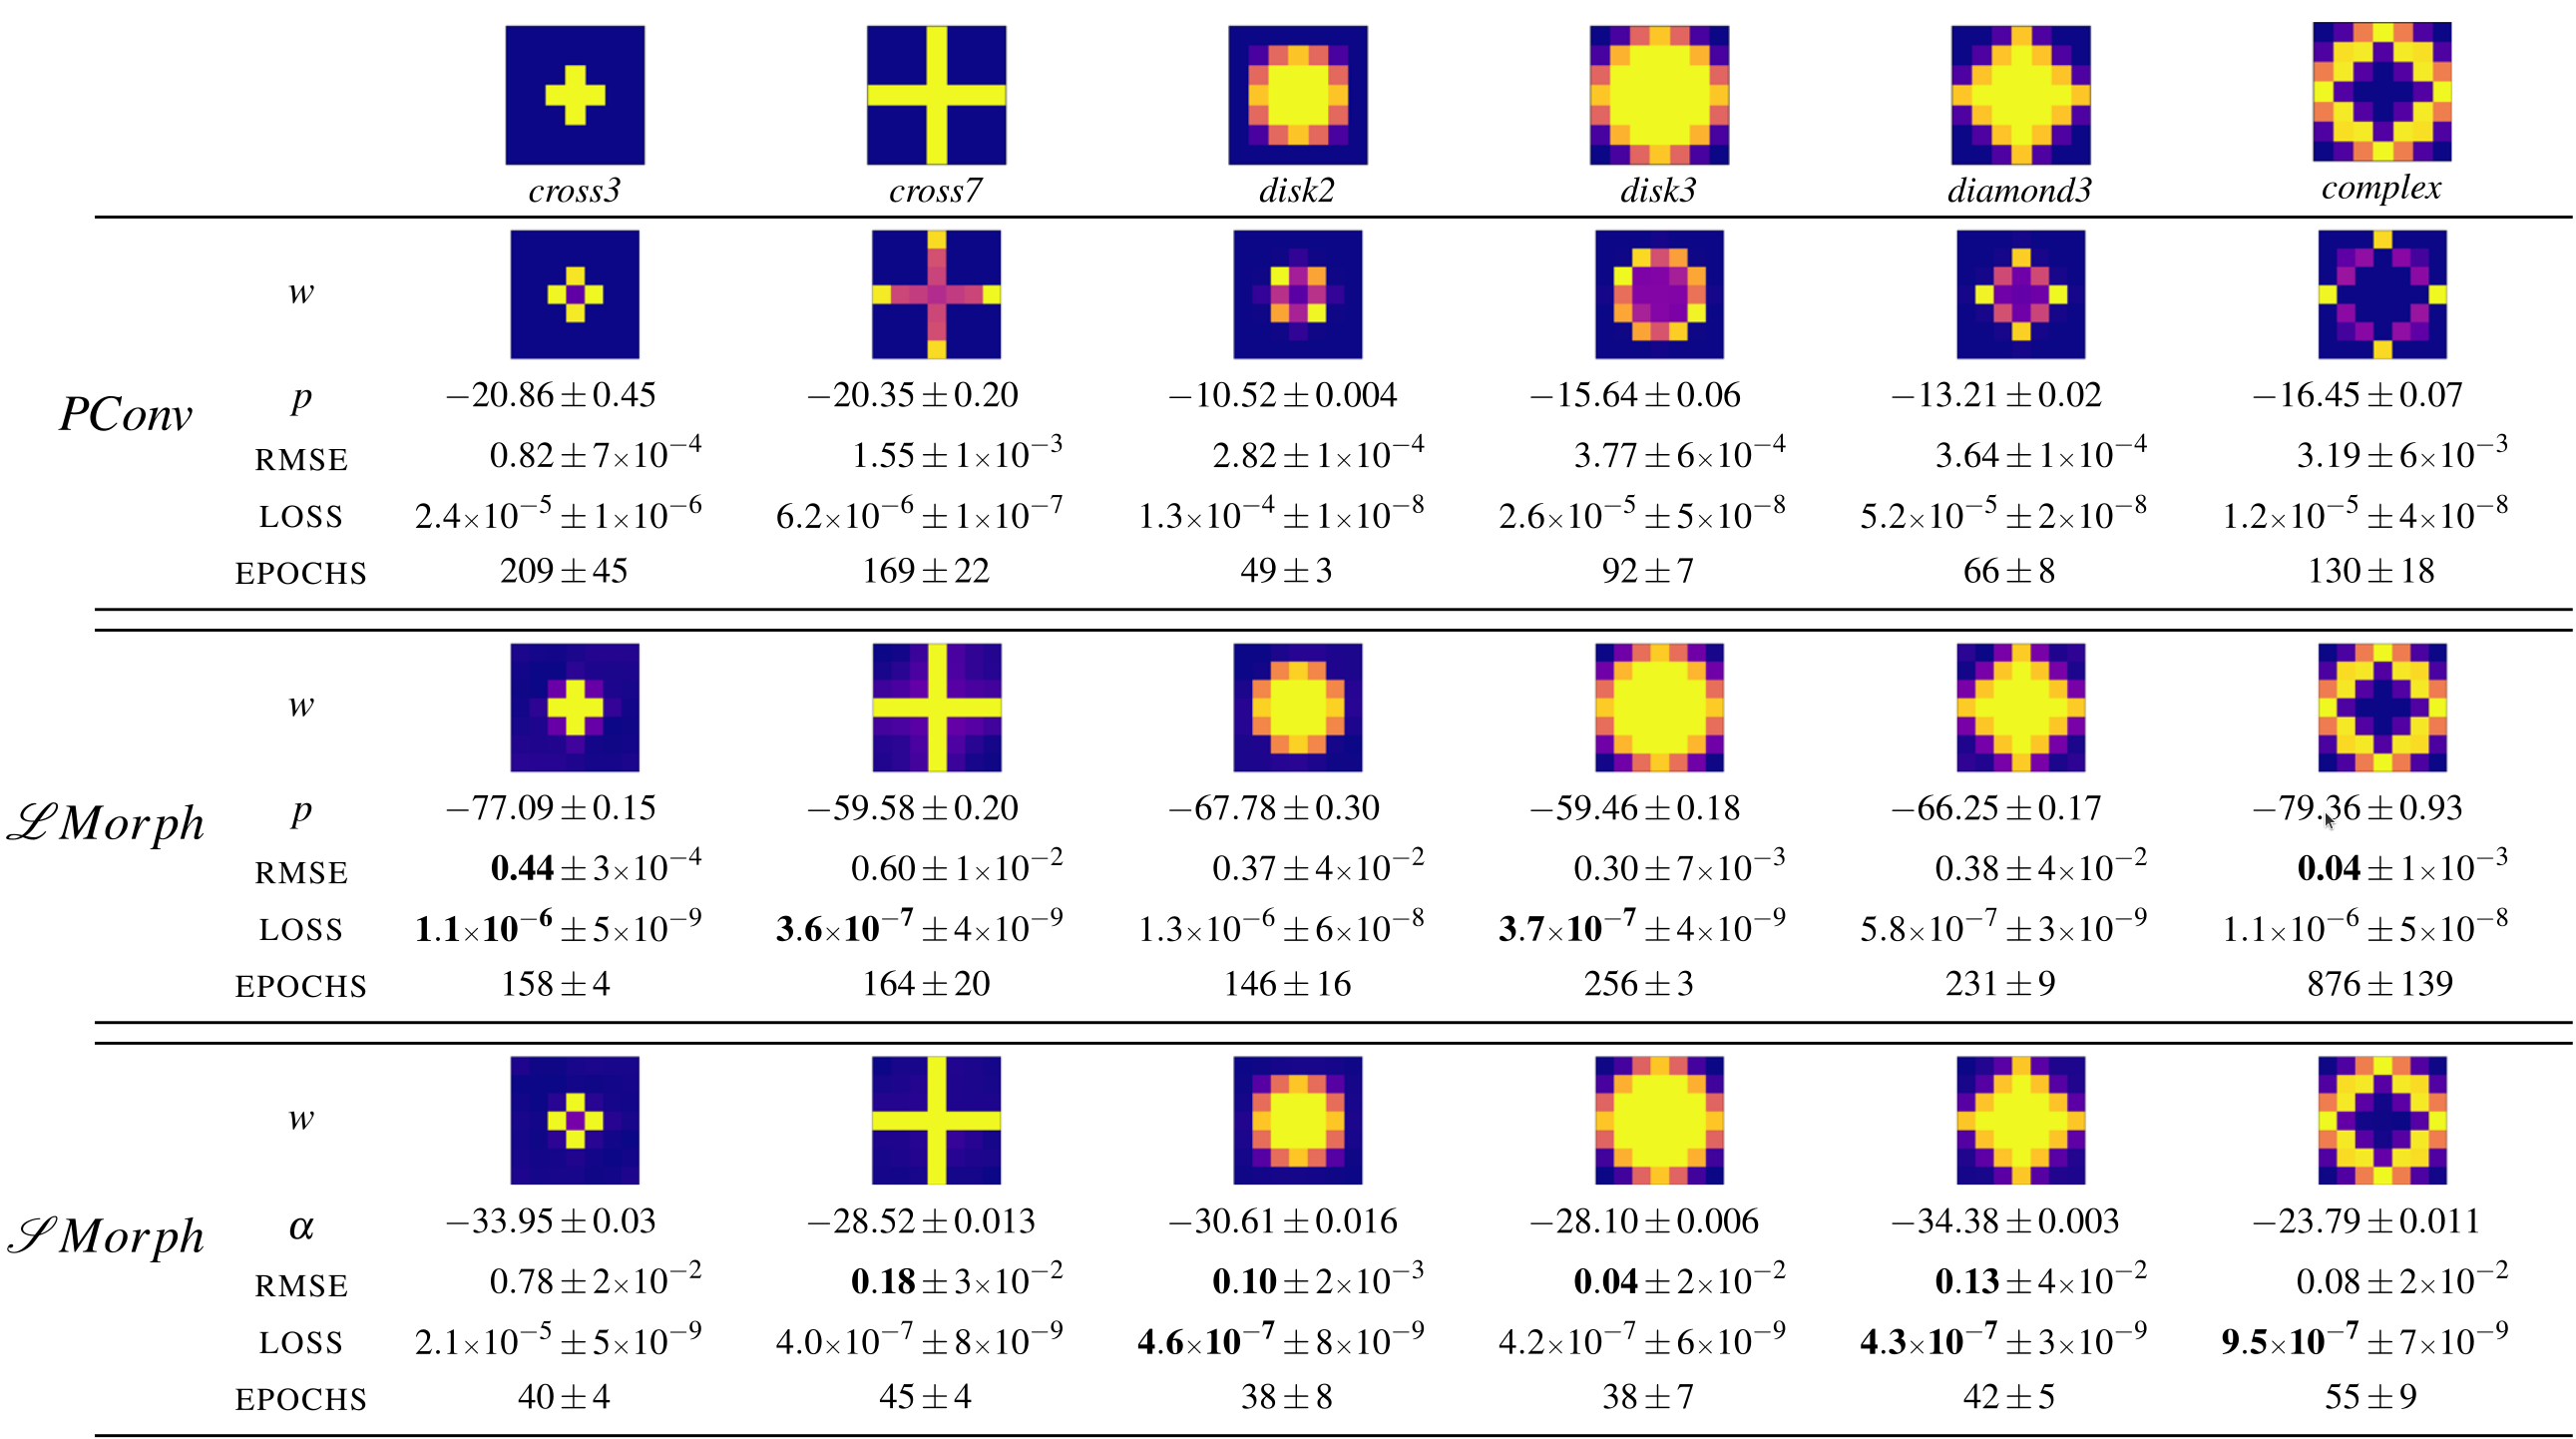
\includegraphics[width=1.00\textwidth]{parts/2-etat_de_lart/D-efficacite_des_reseaux_existant/figures/art_erosion.png}
    \vspace{-2.0mm}
    \caption{ \centering Poids des couches appris et valeur des moyennes et écarts-types des quatre métriques ($p$/$\alpha$, \textit{RMSE}, \textit{loss}, et nombre d'époques) sur cinq runs, pour les trois types de réseaux et les six fonctions structurantes cibles, et pour l'opération cible d'\textbf{érosion}.}
    \label{fig:art_resultats_erosion}
  \end{center}
\end{figure}


\newpage

Dans le deuxième cas, i.e. pour une opération de dilatation avec 1 couche morphologique, on obtient les résultats suivants, sur 5 runs par expérience, fig \ref{fig:art_resultats_dilation} :

% figure
\vspace{2.0mm}
\begin{figure}[ht]
  \begin{center}
    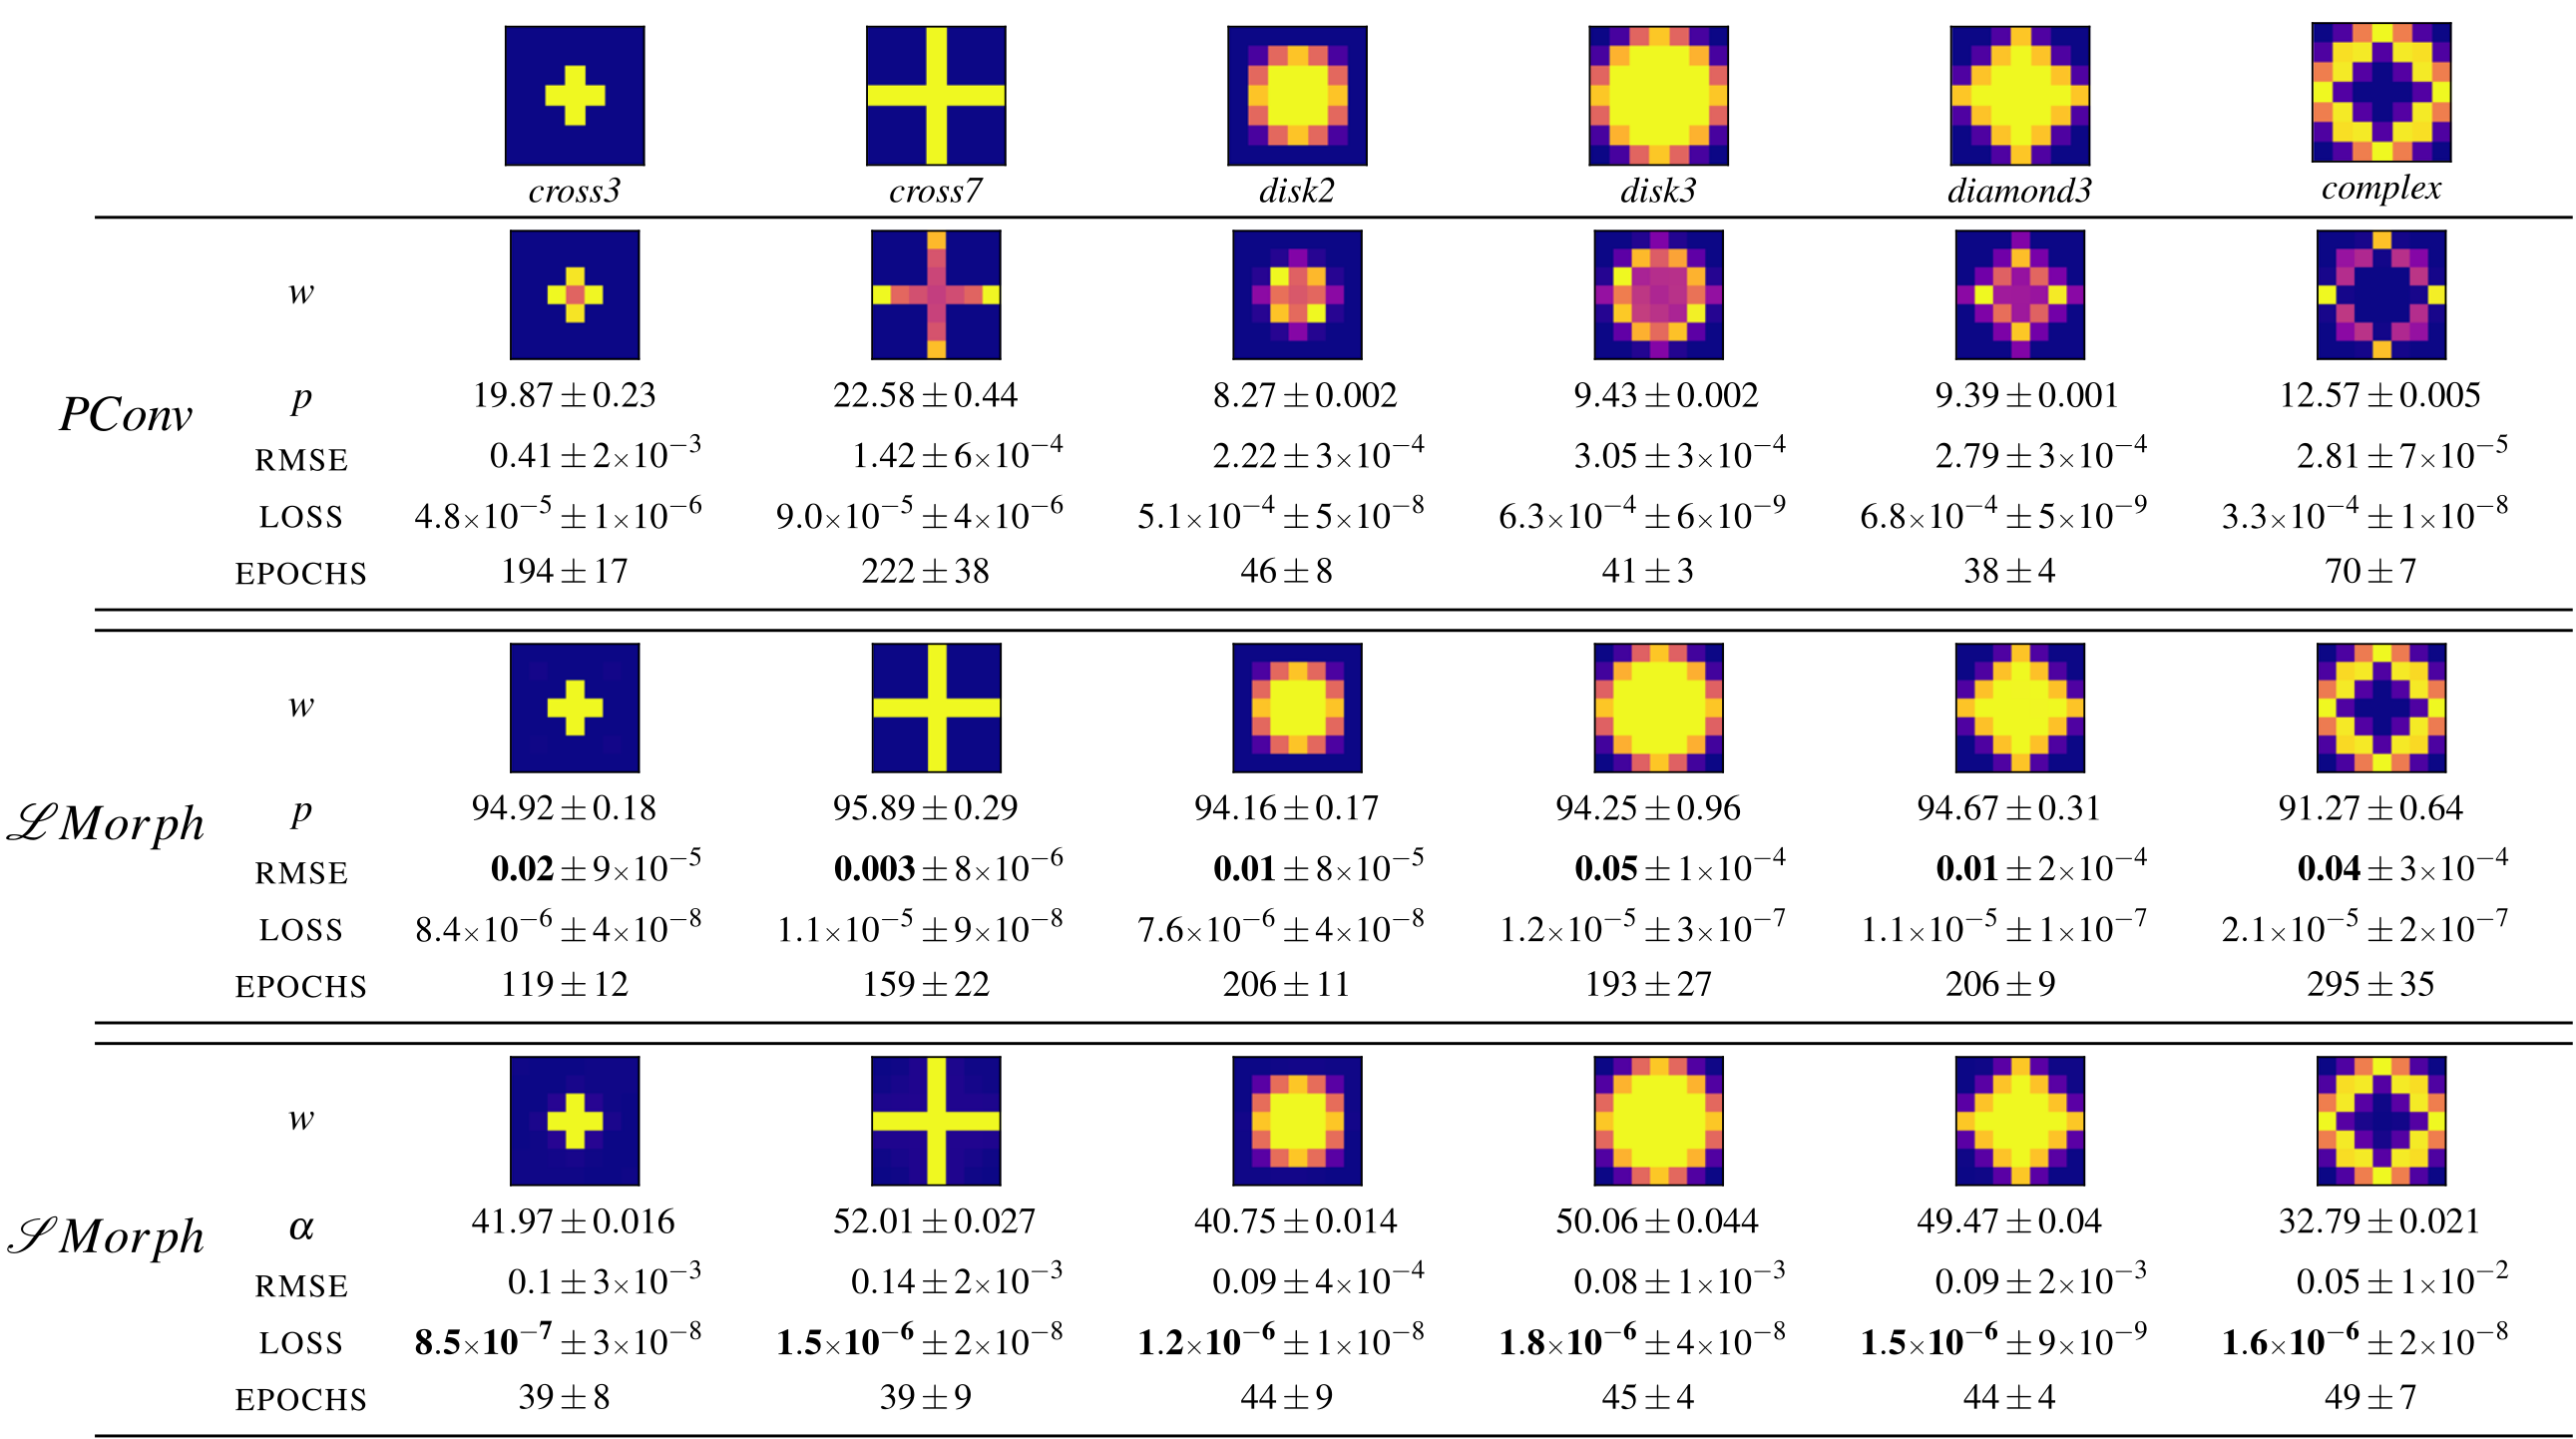
\includegraphics[width=1.00\textwidth]{parts/2-etat_de_lart/D-efficacite_des_reseaux_existant/figures/art_dilation.png}
    \vspace{-2.0mm}
    \caption{ \centering Poids des couches appris et valeur des moyennes et écarts-types des quatre métriques ($p$/$\alpha$, \textit{RMSE}, \textit{loss}, et nombre d'époques) sur cinq runs, pour les trois types de réseaux et les six fonctions structurantes cibles, et pour l'opération cible de \textbf{dilatation}.}
    \label{fig:art_resultats_dilation}
  \end{center}
\end{figure}

\vspace{1.0mm}
A partir des deux figures (fig. \ref{fig:art_resultats_erosion} pour l'ensemble des expériences avec l'érosion, et fig. \ref{fig:art_resultats_dilation} pour celui avec la dilatation), nous pouvons faire les constatations suivantes : \\

%paramètres de contrôle
\noindent D'abord, en examinant la valeur des $p$/$\alpha$ de l'état final des réseaux sur la fig. \ref{fig:art_resultats_erosion} (resp. fig. \ref{fig:art_resultats_dilation}), on constate que les trois types de couches morphologiques parviennent à trouver l'opération morphologique cible, i.e. une érosion (resp. une dilatation), car ces paramètres sont tous négatifs (resp. positifs) et leur amplitude est suffisamment élevée pour considérer l'effet des couches comme véritable opération morphologique. \\

%\vspace{-1.0mm}
\noindent Ensuite, à la fois pour l'érosion et la dilatation, on peut constater que la valeur des RMSE pour l'ensemble des fonctions structurantes cibles est bien plus élevée pour la couche $p$Conv que pour les couches $\mathcal{L}$Morph et $\mathcal{S}$Morph, à l'exception de \textit{cross3}. La forme du noyau des couches $p$Conv est donc moins proche de la cible que les deux autres couches, ce qui peut également être constaté visuellement. La couche $p$Conv semble souffrir d'un certain effet de << creux >> dans la forme de son noyau.


\newpage

\noindent La même chose peut être constatée avec la \textit{loss} des réseaux dans leur état final : elle est bien plus élevée pour la couche $p$Conv, de l'ordre de $10^1$ à $10^2$ fois plus, que pour les couches $\mathcal{L}$Morph et $\mathcal{S}$Morph, qui ont toutes deux le même ordre de grandeur. Ces deux dernières couches sont donc, à la fois pour l'érosion et la dilatation, bien meilleures que la $p$Conv, car elles font de bien meilleures prédictions en moyenne d'après les valeurs de la \textit{loss}. Dans le cadre de la dilatation, fig. \ref{fig:art_resultats_dilation}, la $\mathcal{S}$Morph semble cependant meilleure que la $\mathcal{L}$Morph, d'un ordre de grandeur sur la \textit{loss} en moyenne. \\

\vspace{-1.6mm}
\noindent Le nombre d'époques nécessaire pour atteindre la convergence des réseaux est, pour érosion et dilatation, bien plus faible et régulier sur l'ensemble des expériences pour $\mathcal{S}$Morph que pour $p$Conv ou $\mathcal{L}$Morph. La couche $\mathcal{S}$Morph converge donc plus rapidement et avec plus de régularité que les deux autres couches. 
On remarque également que l'écart-type des métriques sont très faibles, montrant que les réseaux ont convergé sur les 5 cycles d'entraînement (runs) vers la même solution pour les trois couches. \\

%\vspace{-1.0mm}
%Finalement, on peut remarquer que les écarts-types, sur l'ensemble des métriques et des expériences, sont toutes relativement faibles, ce qui indique que les cinq runs (cycles d'entraînement) ont convergé vers la même solution pour les trois couches et les six fonctions structurantes cibles.


\vspace{-1.0mm}
Dans le troisième cas, pour une opération d'ouverture avec 2 couches fig. \ref{fig:art_resultats_opening} : \\
%Dans le troisième cas, i.e. pour une opération d'érosion avec un réseau à 1 couche morphologique, on obtient les résultats de convergence et de caractéristiques suivants, sur 5 runs par expérience, fig \ref{fig:art_resultats_opening} :

% figure
\vspace{-4mm}
\begin{figure}[ht]
  \begin{center}
    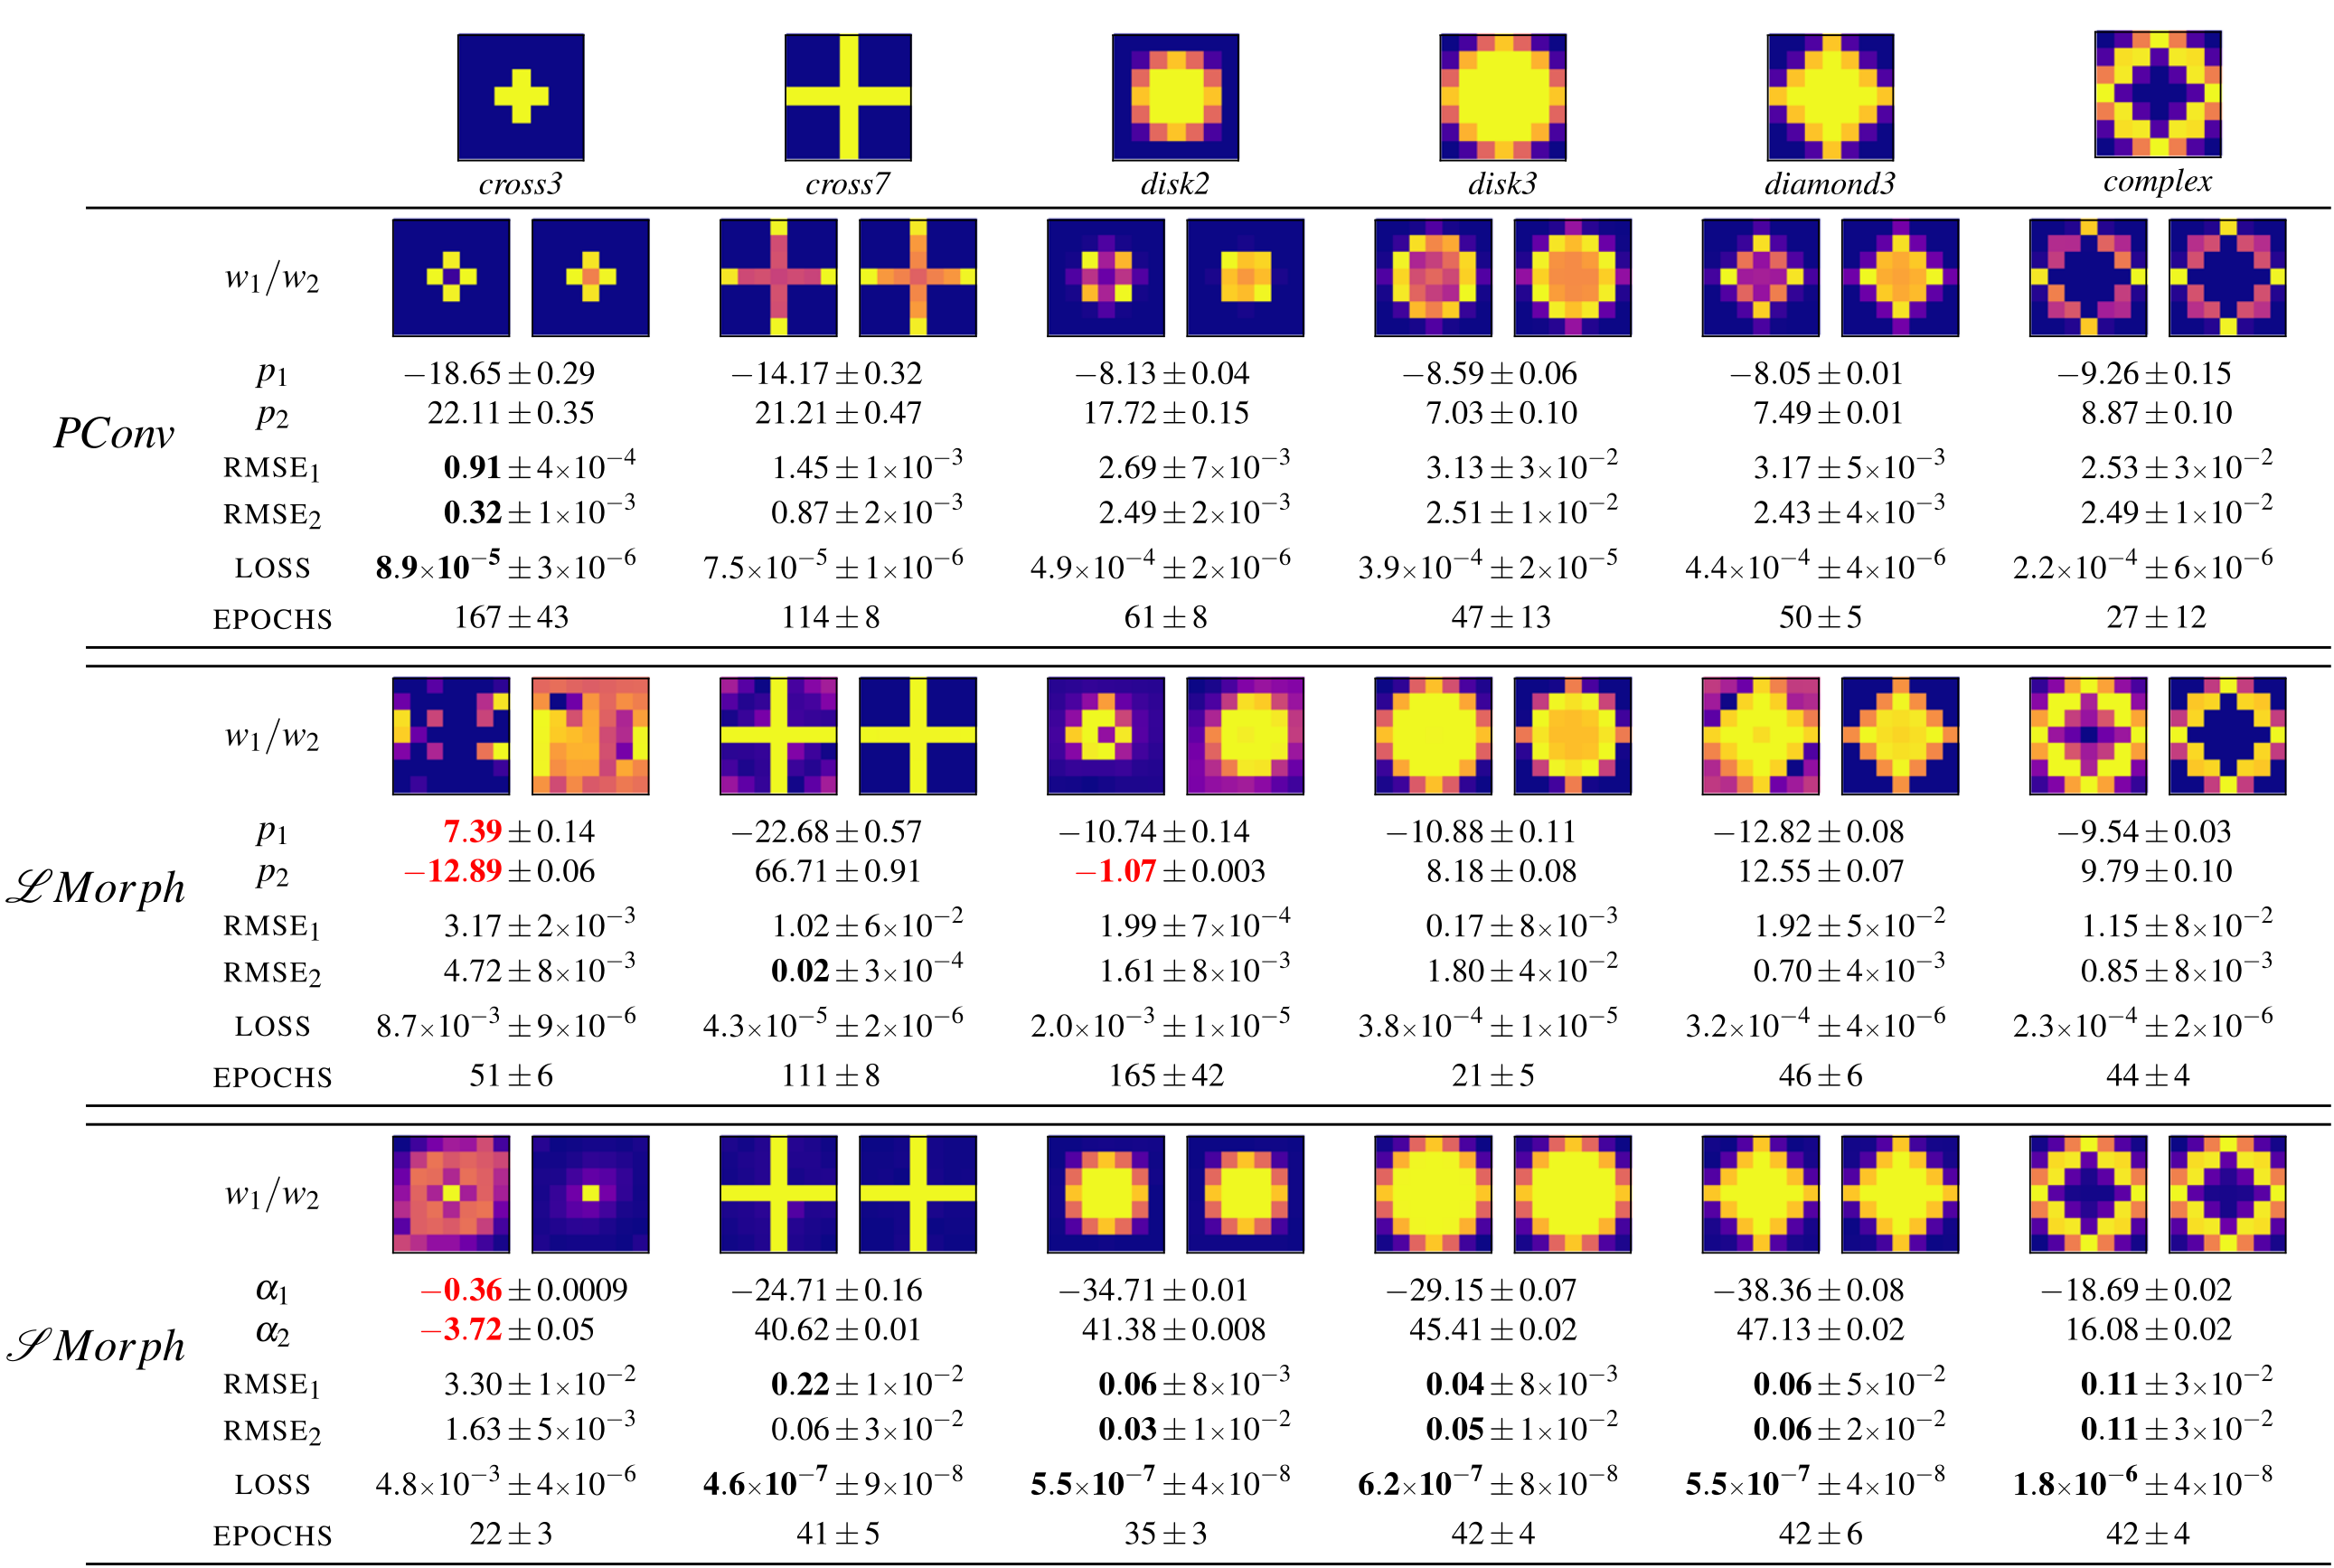
\includegraphics[width=1.00\textwidth]{parts/2-etat_de_lart/D-efficacite_des_reseaux_existant/figures/art_opening.png}
    \vspace{-4.0mm}
    \caption{ \centering Poids des couches appris et valeur des moyennes et écarts-types des quatre métriques ($p$/$\alpha$, \textit{RMSE}, \textit{loss}, et nombre d'époques) sur cinq runs, pour les trois types de réseaux et les six fonctions structurantes cibles, et pour l'opération cible d'\textbf{ouverture}.}
    \label{fig:art_resultats_opening}
  \end{center}
\end{figure}


\newpage

Dans le dernier cas, pour une opération de fermeture avec 2 couches fig. \ref{fig:art_resultats_closing} : \\

% figure
\vspace{-4mm}
\begin{figure}[ht]
  \begin{center}
    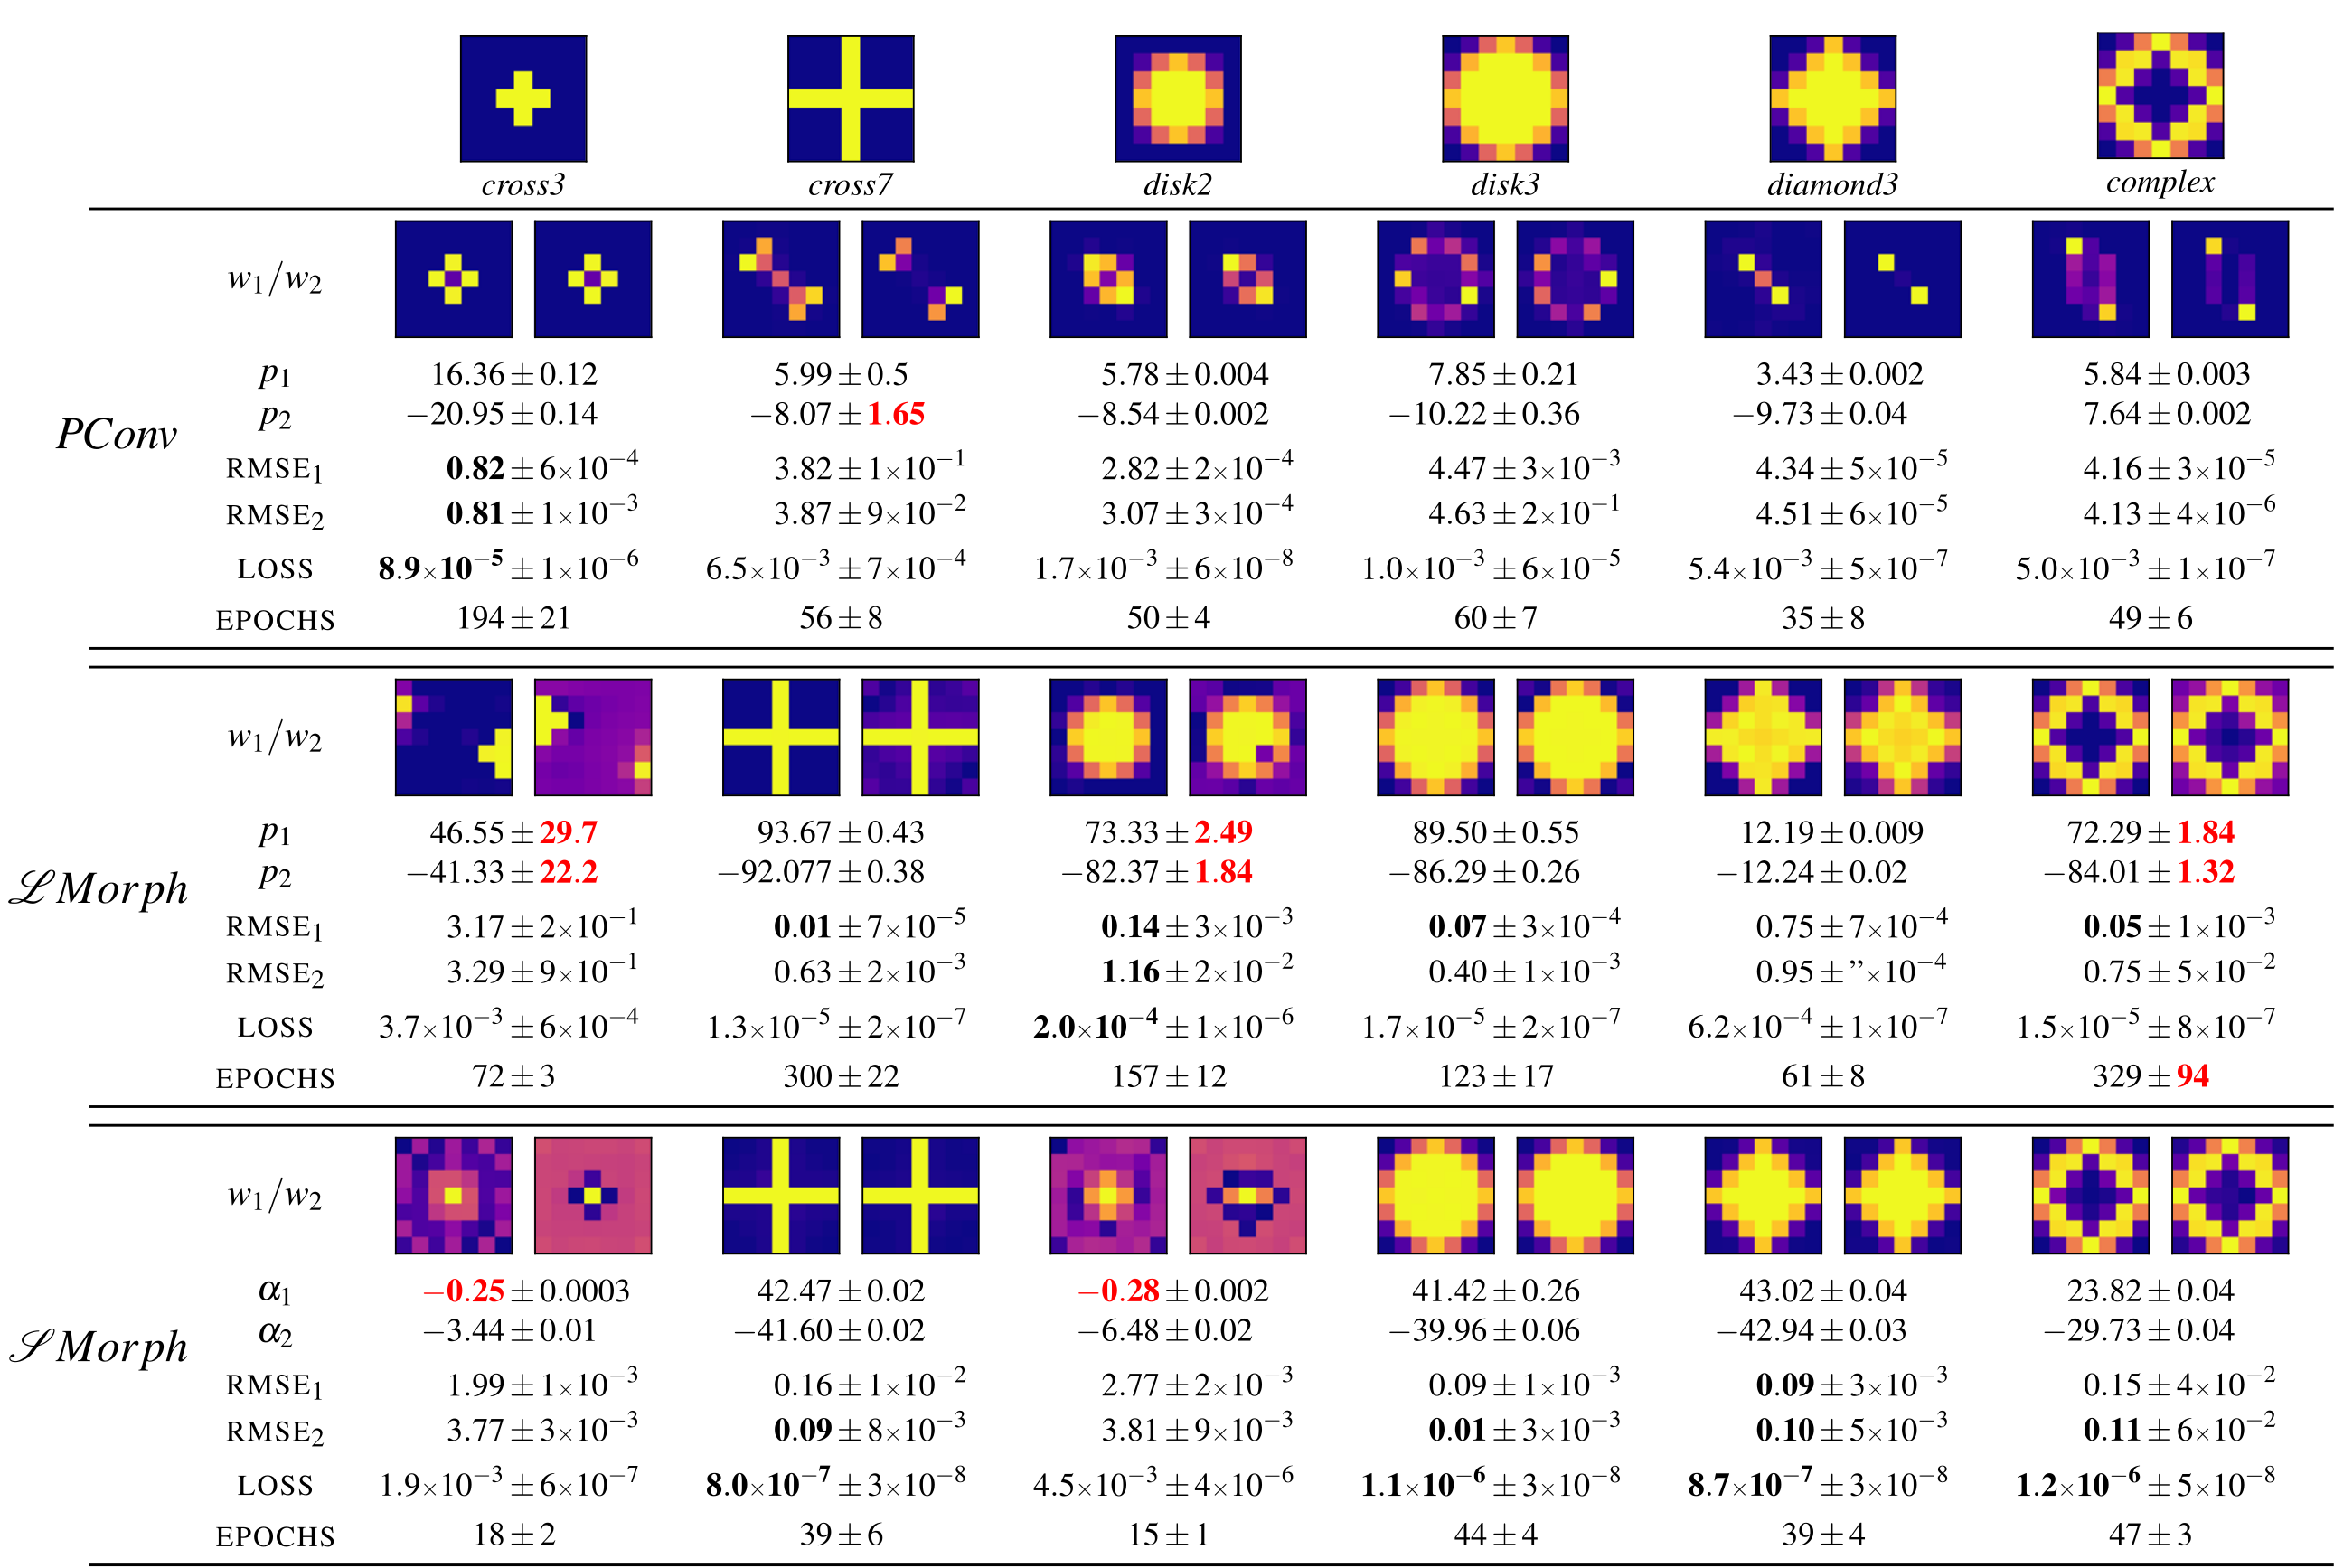
\includegraphics[width=1.00\textwidth]{parts/2-etat_de_lart/D-efficacite_des_reseaux_existant/figures/art_closing.png}
    \vspace{-4.0mm}
    \caption{ \centering Poids des couches appris et valeur des moyennes et écarts-types des quatre métriques ($p$/$\alpha$, \textit{RMSE}, \textit{loss}, et nombre d'époques) sur cinq runs, pour les trois types de réseaux et les six fonctions structurantes cibles, et pour l'opération cible de \textbf{fermeture}.}
    \label{fig:art_resultats_closing}
  \end{center}
\end{figure}


\vspace{-4.2mm}
A partir des deux figures \ref{fig:art_resultats_opening} et  \ref{fig:art_resultats_closing} pour l'ouverture et la fermeture, on remarque la présence évidente d'échecs de convergence. 
Au travers des valeurs de RMSE et des noyaux des couches, on remarque que le réseau $p$ConvNet réussit à plutôt bien deviner la forme de la fonction structurante cible sur l'ensemble des expériences pour l'ouverture, mais pas pour la fermeture où les RMSE et la loss sont tous très élevés. Dans les deux cas, $p$ConvNet souffre toujours de l'effet << creux >>. \\
%Au travers des valeurs des RMSE et de l'aspect visuel du noyau des couches appris, on remarque d'abord que le réseau pConv réussit, pour l'ouverture, plutôt bien à deviner la forme de la fonction structurante cible sur l'ensemble des expériences, mais souffre toujours de l'effet <<creux>>. Pour la fermeture, à l'inverse, les formes apprises sont des échecs, qui s'illustrent à la fois par la haute valeur des RMSE des deux couches pour chaque expérience, et par la valeur bien trop élevée des loss du réseau pConv. \\

\vspace{-1.8mm}
\noindent Hors-mis la cross3, le réseau $\mathcal{L}$MorphNet semble mieux converger que $p$ConvNet sur l'ensemble des expériences, avec des RMSE et des loss bien plus faibles, à la fois pour l'ouverture et la fermeture. Cependant, la forme du noyau des couches n'est pas parfaite, et varie beaucoup entre la première et la seconde couche du réseau, ce qui n'est pas le cas pour le réseau $\mathcal{S}$MorphNet qui, hors-mis avec le disk2 (fermeture), est meilleur encore et ne présente pas cette disymétrie de noyau entre les deux couches du réseau. $\mathcal{S}$MorphNet surpasse presque toujours $p$ConvNet et $\mathcal{L}$MorphNet en termes de RMSE, de loss et de nombre d'époques, pour à la fois l'ouverture et la fermeture.
%\noindent En-dehors de la cross3, le réseau LMorph semble mieux converger que pConv sur l'ensemble des expériences, avec des valeurs de RMSE et de loss bien plus faibles que ce dernier, à la fois pour l'ouverture et la fermeture. Cependant, la forme du noyau des couches est loin d'être parfaite, et varie beaucoup entre la première et la seconde couche du réseau. Le réseau SMorph, quant à lui, semble meilleur encore que LMorph, hors-mis le cas du disk2 pour la fermeture, avec des RMSE et des loss plus faibles encore, et des formes de noyaux plus proches de la cible et plus stables entre la première et la seconde couche. \\

%%% \noindent En se penchant sur les valeurs des paramètres de contrôle $p$/$\alpha$, on remarque que, dans les cas d'échec, les couches des réseaux n'ont pas convergé vers la bonne opération (entre érosion et dilatation), avec des $p$/$\alpha$ de signe opposé à ce qu'ils devraient prendre, et de faible amplitude, comme c'est le cas par exemple avec cross3 (ouverture et fermeture) pour les réseaux LMorph et SMorph, ou encore avec disk2 (fermeture) pour SMorph. Le signe vers lequel tendent les $p$/$\alpha$ des deux couches d'un réseau semblent jouer un rôle conséquent dans l'échec de convergence de ce dernier. \\

%\noindent Enfin, notamment pour la fermeture, les réseaux semblent peu stables en termes de résultats de convergence, comme le montrent les fortes valeurs d'écart type pour les métriques quantitatives rapportées. \\

%\noindent À l'exception des cas d'échec sur cross3 et disk2, on remarque finalement que SMorph surpasse presque systématiquement PConv et LMorph en termes de RMSE pour les deux couches, en terme de loss à la convergence, et terme de nombre d'époques d'entraînement, et ce à la fois pour l'ouverture et la fermeture. \\
